
The results were obtained using the
PDF4LHC15{\tt\_}nlo{\tt\_}30{\tt\_}pdfas~\cite{Butterworth:2015oua,CT14,MMHT14,NNPDF}
parton distribution functions interfaced to our code via
LHAPDF~\cite{Buckley:2014ana}, along with the corresponding value for
$\alpha_s$.  The masses of the Higgs boson and the top quark have been
fixed, as in the virtual amplitude, to $m_h=125$\,GeV, $m_t=173$\,GeV,
respectively. Their widths have been set to zero.   
Jets are clustered with the
anti-$k_T$ algorithm~\cite{Cacciari:2008gp} as implemented in the
{\tt fastjet} package~\cite{Cacciari:2005hq, Cacciari:2011ma}, with jet
radius $R=0.4$ and a minimum transverse momentum 
$p_{T,min}^{\rm{jet}}=20$\,GeV.  The scale uncertainties are
estimated by varying the factorisation/renormalisation scales
$\mu_{F}, \mu_{R}$. The scale variation bands 
represent scale variations around the central scale $\mu_0 =\mhh/2$, with
$\mu_{R,F}=c_{R,F}\,\mu_0$, where $c_R=c_F= \{0.5,0.5\}$ and $c_R=c_F= \{2,2\}$.
For the case $\lambda=1$ we checked that the bands obtained from these variations coincide with the bands resulting from 7-point scale variations.

\subsection{Total cross sections at different values of the trilinear coupling}

In Table \ref{tab:sigmatot} we list total cross sections at 14\,TeV and 27\,TeV for various values of the trilinear Higgs coupling $\lambda$. 
\begin{table}[htb]
\begin{center}
%\setlength{\extrarowheight}{3.0pt}
\begin{tabular}{| c | c | c |c|c|}
%\Xhline{2\arrayrulewidth}
\hline
&&&&\\
$\lambda_{\mathrm{BSM}}/\lambda_{\mathrm{SM}}$ & $\sigma_{\rm{NLO}}@14 \mathrm{TeV}$\,[fb] & $\sigma_{\rm{NLO}}@27 \mathrm{TeV}$\,[fb] &K-fac.@14TeV&K-fac.@27TeV\\
&&&&\\
\hline
1& 32.88$^{+13.5\%}_{-12.5\%}$&127.7$^{+11.5\%}_{-10.4\%}$ &1.66&1.62\\
\hline
2 & 14.91 &  59.10 & 1.58 & 1.52\\
\hline
2.4 & 13.81& 53.67 & 1.65 & 1.60\\
\hline
3& 19.82 & 69.84 & 1.97 & 1.89\\
\hline 
5 & 95.22$^{+19.7\%}_{-11.5\%}$& 330.61 & 2.21 & 2.18\\
\hline 
0 & 73.64$^{+15.4\%}_{-13.4\%}$& 275.29& 1.79 & 1.78 \\
\hline 
-1 & 136.91$^{+16.4\%}_{-13.9\%}$& 504.9 & 1.87 & 1.83\\
\hline
%\Xhline{2\arrayrulewidth}
\end{tabular}
\end{center}
\caption{Total cross sections for Higgs boson pair production at full NLO. The given uncertainties are scale uncertainties. 
\label{tab:sigmatot}}
\end{table}
Table~\ref{tab:sigmatot} shows that the K-factors vary substantially as functions of the trilinear coupling.
This fact is illustrated in Fig.~\ref{fig:Kfacvariation}, showing that the K-factor takes values between 1.57 and 2.16
if the trilinear coupling is varied between $-5\leq \chhh\leq 12$.

\begin{figure}[htb]
  \centering
    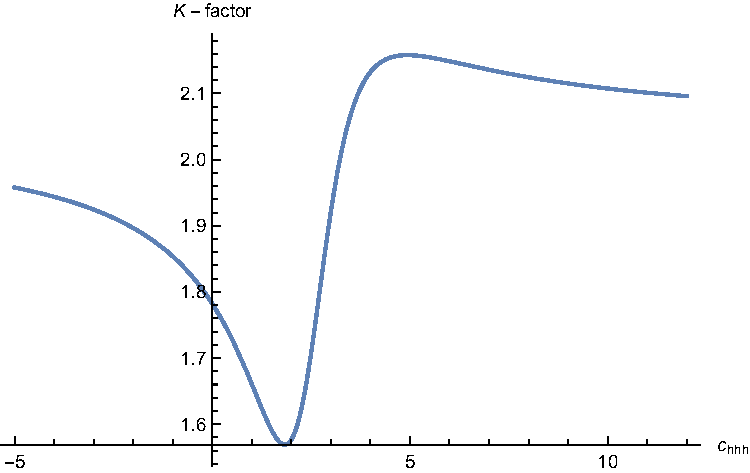
\includegraphics[width=0.4\textwidth]{plots/Kfac_varlambda.pdf}
%  \includegraphics[width=\textwidth]{plots/}
%    \caption{\label{fig:lambda_large_27}}
\caption{Variation of the NLO K-factor with the trilinear coupling, $\sqrt{s}=14$\,TeV.}
\label{fig:Kfacvariation}
\end{figure}


\subsection{Differential cross sections}

In Figs.~\ref{fig:lambda_small} and ~\ref{fig:lambda_large} we show the $\mhh$ distribution for various values of $\chhh=\lambda_{\mathrm{BSM}}/\lambda_{\mathrm{SM}}$. 
The ratio plots show the differential K-factors. 

\begin{figure}[htb]
 \begin{subfigure}{0.495\textwidth}
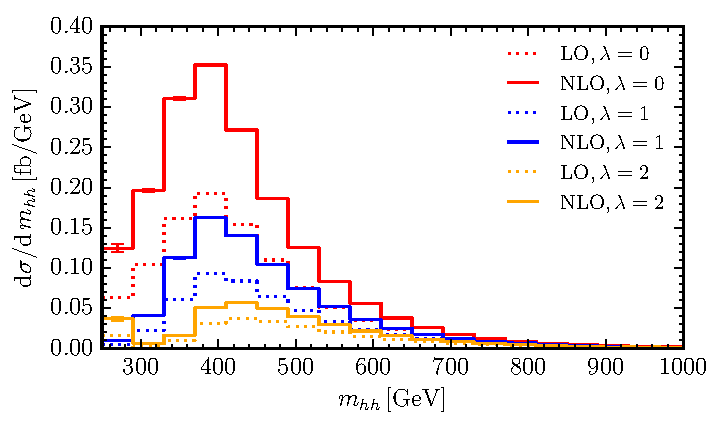
\includegraphics[width=\textwidth]{plots/mhh_Kfac_14TeV_varylambda_small.pdf}
%    \vspace{\TwoFigBottom em}
 \caption{Higgs boson pair invariant mass distributions for various values of $\lambda$ (relative to $\lambda_{\mathrm{SM}}$)  at 14\,TeV.}
\label{fig:lambda_small}
\end{subfigure}
\hfill
\begin{subfigure}{0.495\textwidth}
    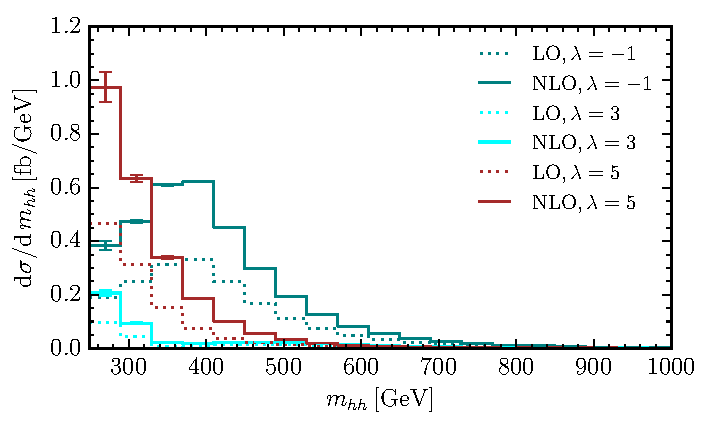
\includegraphics[width=\textwidth]{plots/mhh_Kfac_14TeV_varylambda_large.pdf}
\caption{Higgs boson pair invariant mass distributions for $\lambda/\lambda_{\mathrm{SM}}=-1,3,5$)  at 14\,TeV.}
\label{fig:lambda_large}
\end{subfigure}
\label{fig:lambdavar14TeV}
\end{figure}


%\begin{figure}[ht]
%\begin{center}
%  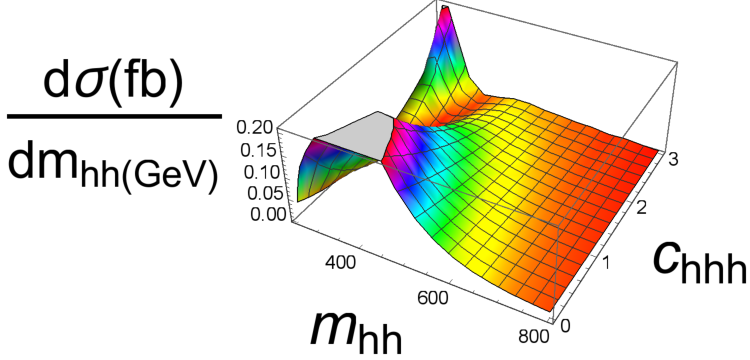
\includegraphics[width=0.55\textwidth]{plots/3D_mhh_chhh.pdf}    
%\end{center}
%\caption{3-dimensional visualisation of the $\mhh$ distribution at 14\,TeV, as a function  $\chhh$ and $\mhh$. The units on the y-axis are [fb/GeV].}
%\label{fig:chhh_3D}
%\end{figure}
%Fig.~\ref{fig:chhh_3D} shows the Higgs boson pair invariant mass
%distributions at NLO as a function of $\chhh$  as 3-dimensional heat maps.
%The other couplings are fixed to their SM values.
 
 

